\documentclass{article}
\usepackage[14pt]{extsizes}
\usepackage[T2A]{fontenc}
\usepackage[utf8]{inputenc}
\usepackage[english, russian]{babel}
\usepackage[left=3cm,right=1.5cm,top=2cm,bottom=2cm]{geometry}
\usepackage{hyperref}
\usepackage{amsmath}
\usepackage{cleveref}
\usepackage{caption}


\usepackage{graphicx}

%\полуторный интервал
\usepackage{setspace}
\onehalfspacing

%простое дерево
\usepackage{dirtree}

%формулы
\usepackage{mathtools}
\usepackage{amsfonts}
% \everymath{\displaystyle}

%красные строки (не рекомендуется)
% \parindent = 1,25cm
% \usepackage{indentfirst}

\begin{document}
%\input{title}
\tableofcontents
\newpage

\section{System architecture}


\subsection{Обработка гомогенных и гетерогенных данных}
\begin{quote}
    Homogeneous Data Structures: This type can only store a single type of data inside them(integer, character, etc.), Heterogeneous Data Structures: This type can store more than one type of data at the same.
\end{quote}
Основным принципом работы классических баз данных является обращение к памяти на физическом устройстве.
с помощью индекса (например хеш функции). Основой таких баз данных является реляционная алгебра.\\
\textbf{Реляционные базы данных} используют таблицы для хранения строго структурированных данных.\\
\textbf{Структурированные данные} предполагают наличие определенной схемы (определяется при создании базы данных) и типа данных.\\\\
Но с развитием реляционных баз данных были введены новые полуструктурированные данные, которые могут содержать наборы данных с бесконечными(динамическими) значениями, состоять из других объектов данных. С дальнейшем
развитием технологий возникает понятие NoSQL, которые могут работать с слабоструктурированными и неструктурированными объектами. \textbf{Например: } фильм, аудиофайл.\\
Один из таких типов данных это поток данных записываемых в базу данных.\\
\textbf{Поток данных} - это поток данных с изменяемым числом записей в секунду(any unit of time). Особенностью таких данных является то что обрабатывать такие данные можно только последовательно.\\\\
На изображении \ref{img1} показана система аукциона представляемая потоком данных. Ставки имеют объем в валюте и временю метку. Затем будет выбран пользователь что сделал наибольшую ставку. А поток данных можно использовать для дальнейшего анализа.
\newpage
\begin{figure}[h]
    \centering
    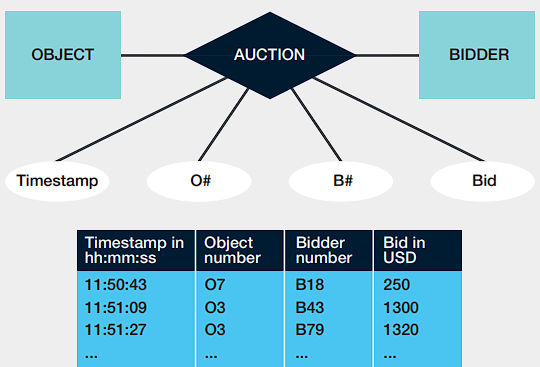
\includegraphics[width=0.7\textwidth]{images/datastream.png}
    \caption{Поток данных}
    \label{img1}
\end{figure}
\textbf{Неструктурированные данные} - данные без структуры, например снимки с спутников, музыкальные файлы. Чаще всего такие данные возникают в процессах big data. Хранилища данных для таких типов являются NoSQL.


\subsection{Структуры хранения и доступа}
\begin{quote}
    Storage and access structures for relational and nonrelational database systems should 
    be designed to manage data in secondary storage as efficiently as possible.
\end{quote}

\subsubsection{Структуры: индекс, дерево}
\textbf{Индекс атрибута} это структура, которая эффективно предоставляет для каждого значения атрибута, внутренний адрес для всех записей имеющих такое значение атрибута.\\
\textbf{Пример:} сортированная нумерация, отсортированные по алфавиту строки.\\\\
\textbf{Структуры вида дерево} позволяют хранить записи или индексы для увеличения эффективности. Для получения записи необходимо выполнить операцию поиска по дереву.
В классической реализации дерево состоит из корневого узла и внутренних узлов, каждый из которых имеет 2 поддерева(бинарное дерево).
Проблема таких деревьев в высокой скорости роста высоты, а следовательно и количества запросов для доступа к данным. Для решения этой проблемы деревья предложено расширять в ширину а не высоту.
Одной из структур реализующих этот подход является B-tree.\\
\textbf{B-tree} - дерево в котором каждый узел имеет более 2ух поддеревьев. Где внутренние узлы и листья дерева не пусты.
B-tree $n$ ого порядка назовем дерево если:
\begin{enumerate}
    \item оно полностью сбалансировано (путь от корня до каждого листа имеет одинаковую длину)
    \item каждый внутренний узел имеет хотя бы $n$ и максимум $2*n$ вхождений в его data page.
\end{enumerate}
На рисунке \ref{img2} показано:
\begin{enumerate}
    \item Как таблица обращается в дерево индексов. Для нашего дерева $n = 2$ значит мы храним максимум 4 элемента в узле.
    \item Затем производится попытка добавить элемент, но т.к размер дерева $n = 2$ дерево получает новый слой, и элементы разделяются на 2 поддерева относительно медианного элемента.
    \item На третьем этапе, показано как дерево изменяет свою форму при заполнении узла в поддереве, но когда его относительной корневой узел не заполнен.
\end{enumerate} 
\begin{figure}[h]
    \centering
    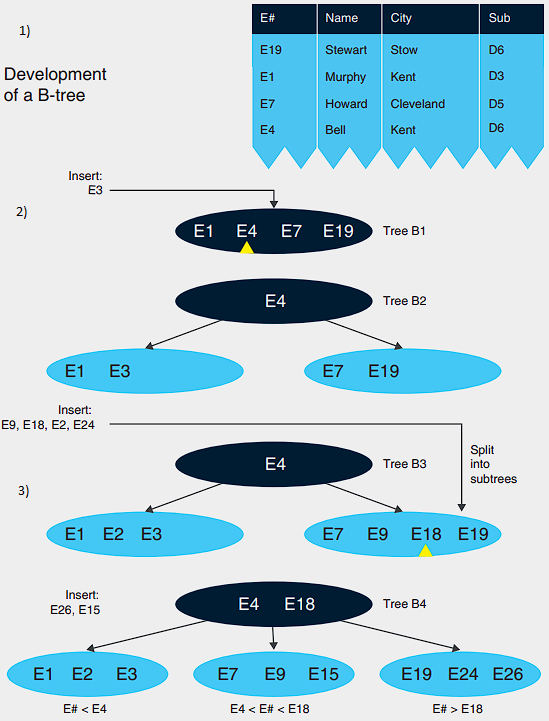
\includegraphics[width=0.7\textwidth]{images/btree.png}
    \caption{B-tree в динамике}
    \label{img2}
\end{figure}
\newpage
Время доступа используя B-tree напрямую зависит от его высоты. Как было показано высоту можно компенсировать увеличиваем количества поддеревьев.

\subsubsection{Методы хеширования}
\textbf{Хеширование} - определение адреса с помощью хеш функции.\\
\textbf{Хеш функция} - отображает множество ключей в непрерывное множество адресов. И удоволетворяет:
\begin{enumerate}
    \item Отображение можно повторить с помошью простых вычислений.
    \item Полученный адрес должен быть одинаково распределен в адресном пространстве.
    \item Вероятность коллизий одинакова для всех ключей.
\end{enumerate}
\textbf{Пример:} $H(k) = k \: mod \: p$ взятие модуля для определения адреса или номера страницы.\\
\textbf{Переполнение} - ситуация когда отоброжение в определенный адрес переполняет число возможных значений внутри этого адреса. Для борьбы с такой ситуацией используют динамические хеш функции, изменяют размер адресного множества без необходимости переносить записанные значения.

\subsubsection{Согласованное хеширование}
В технологиях болших данных применяются хеш функции для отображения ключ-значение на различные узлы в компьютерной сети. Согласованное хеширование предполагает вычисление адреса для узла и для хранилища объекта.\\
На рисунке \ref{img3} показано пространство в виде окружности, где с помошью хеш функции устанавливаются узлы на окружности, затем объекты типа ключ-значение наносятся на окружность.
Для определения принадлежности к узлу достаточно найти следующий узел проходя по часовой стрелке окружности. 
\begin{figure}[h]
    \centering
    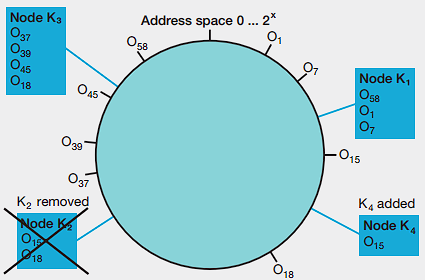
\includegraphics[width=0.7\textwidth]{images/consistent_hash.png}
    \caption{Согласованное хеширование}
    \label{img3}
\end{figure}
\newpage
Основным достоинтсвом такой системы является гибкость при добавлении узлов, т.к нам не нужно вычислять новые адреса при изменении структуры нашего хранилища.

\subsubsection{Структуры данных размерности порядка > 1}
\textbf{Ключ K размерности n} - набор из n атрибутов необходимый для однозначного доступа к записи. $K \in \mathbb{R}^n$\\
\textbf{Ключ K} - симметричный, если доступ к данным не зависит от порядка элементов в ключе.\\\\
Одна из наиболее важных многомерных структур - grid file.\\
\textbf{Grid file:}
\begin{enumerate}
    \item Разбивает пространство ключей на сетку объединяя некоторые ключи в одно множество - bucket.
    \item Предоставляет доступ к данным путем обращеня к элементу ключа внутри набора(bucket).
\end{enumerate}
Такая структура позволяет эффективно организовывать многомерный поиск. Благодоря объединеню некоторых элементов в подмножество. Набор таких множеств образует сетку в $n$ мерном пространстве\\
На рисунке \ref{img4} показана структура, где пространство разделено на сетку. Для обращения нужно выполнить поиск по индексам сетки а затем множеству внутри нужного bucket.
\begin{figure}[h]
    \centering
    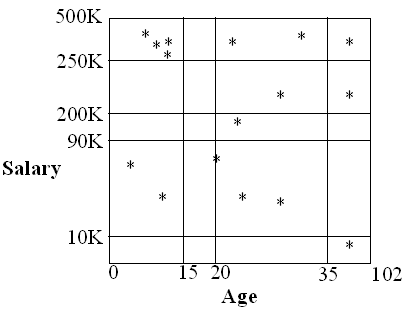
\includegraphics[width=0.7\textwidth]{images/grid.png}
    \caption{grid file}
    \label{img4}
\end{figure}
\\
В настоящее время данная структура активно исследуется, но не используется активно.


\subsection{Перевод и оптимизация реляционных запросов}
\end{document}